Let $X$ be a random variable and the CDF $F_X(x)$ be defined as
\begin{align}
    F_X(x) =
\begin{cases}
    \frac{x}{2} & 0\leq x<\frac{1}{2} \\
    x & \frac{1}{2}\leq x\leq 1
\end{cases}
\end{align}
\begin{figure}[h]
    \centering
    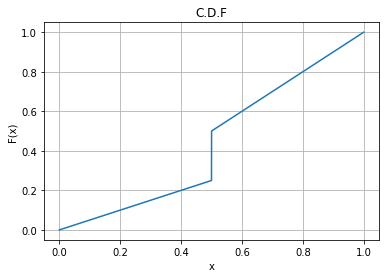
\includegraphics[width=\columnwidth]{solutions/ec/72/Assignment_2_AI1103.png}
    \caption{Graph representing CDF}
    \label{ec72:fig:1}
\end{figure}
The probability of getting a number in $\left[0,\frac{1}{2}\right)$, i.e, $x=\frac{1}{2}^-$ is
\begin{align}
    F_X\brak{\frac{1}{2}^-} &= \frac{\frac{1}{2}}{2}\\
    F_X\brak{\frac{1}{2}^-} &= \frac{1}{4}
\end{align}\\
The probability of getting a number in $\left[0,\frac{1}{2}\right]$, i.e, $x=\frac{1}{2}$ is
\begin{align}
    F_X\brak{\frac{1}{2}} &= \frac{1}{2}
\end{align}\\
Therefore, the probability of getting $\cbrak{\frac{1}{2}}$ is
\begin{align}
    \pr{X=\frac{1}{2}} &= F_X\brak{\frac{1}{2}} - F_X\brak{\frac{1}{2}^-} \\
    \pr{X=\frac{1}{2}} &= \frac{1}{2} - \frac{1}{4} \\
    \pr{X=\frac{1}{2}} &= \frac{1}{4}
\end{align}
